%%%%%%%%%%%%%%%%%%%%%%%%%%%%%%%%%%%%%%%%%%%%%%%%%%%%%%%
% A template for Wiley article submissions.
% Developed by Overleaf. 
%
% Please note that whilst this template provides a 
% preview of the typeset manuscript for submission, it 
% will not necessarily be the final publication layout.
%
% Usage notes:
% The "blind" option will make anonymous all author, affiliation, correspondence and funding information.
% Use "num-refs" option for numerical citation and references style.
% Use "alpha-refs" option for author-year citation and references style.
\PassOptionsToPackage{author-year,initials,nobysame}{amsrefs}
\documentclass[ams-refs]{wiley-article}
% \documentclass[blind,ams-refs]{wiley-article}

% Add additional packages here if required
\usepackage{siunitx}

% added LG
\usepackage{lineno}
\usepackage{todonotes}
\usepackage{verbatim}

% Update article type if known
\papertype{Original Article}
% Include section in journal if known, otherwise delete
\paperfield{Journal Section}

\title{Leveraging Prediction Errors originating in Midline Cingulate and Parieto-occipital EEG Sources to Classify User Experience Disruptions in AR/VR}

% alternative titles
% sources capture sensory prediction errors but are not modulated by ongoing motor behavior
% Single-trial regression mapping biomechanics to event-related brain dynamics: hand movement velocity impacts posterior cingulate activity in sensory-motor coupling
% Not reaching your target: prediction errors are modulated by hand movement speed, haptic feedback 
%mobi using motion parameters to inform brain dynamic analysis
%Sensory-motor integration in anterior cingulate cortex: visuo-haptic mismatches and the impact of hand movement speed
% single-trial analysis elucidating spatio-temporal multisensory integration in parietal EEG sources

% List abbreviations here, if any. Please note that it is preferred that abbreviations be defined at the first instance they appear in the text, rather than creating an abbreviations list.
%\abbrevs{ABC, a black cat; DEF, doesn't ever fret; GHI, goes home immediately.}

% Include full author names and degrees, when required by the journal.
% Use the \authfn to add symbols for additional footnotes and present addresses, if any. Usually start with 1 for notes about author contributions; then continuing with 2 etc if any author has a different present address.
\author[1\authfn{1}]{Lukas Gehrke}
\author[1]{Pedro Lopes PhD}
\author[1]{Marius Klug}
\author[2]{Sezen Akman}
\author[1,3,4,5]{Klaus Gramann PhD}

%\contrib[\authfn{1}]{Equally contributing authors.}

% Include full affiliation details for all authors
\affil[1]{Biopsychology and Neuroergonomics, Institute of Psychology and Ergonomics, TU Berlin, Berlin, Berlin, 10623, Germany}
\affil[2]{Department, Institution, City, State or Province, Postal Code, Country}

\corraddress{Lukas Gehrke, Biopsychology and Neuroergonomics, TU Berlin, Berlin, Berlin, 10623, Germany}
\corremail{lukas.gehrke@tu-berlin.de}

\presentadd[\authfn{1}]{Biopsychology and Neuroergonomics, Institute of Psychology and Ergonomics, TU Berlin, Berlin, Berlin, 10623, Germany}

\fundinginfo{This research was supported by a grant from the German Federal Ministry of Education and Research (01GQ1511) to KG}

% Include the name of the author that should appear in the running header
\runningauthor{Gehrke et al.}

\begin{document}
\maketitle

% added LG
\linenumbers

% % add abstract
\begin{abstract}

Neural interface technology holds significant promise to track user experience implicitly. Today, it finds increasing application in VR/AR as it allows user assessment without breaking the immersive experience. In VR, designing immersion is the key challenge. Unfortunately, the established metric to assess the effectiveness of immersive VR simulations relies on questionnaires. In this work, we present a complimentary metric based on a Brain-Computer Interface. For the metric to be useful beyond prototypical applications, the neural signal employed must be reliable. Hence, it is beneficial to target the signal's cortical origin directly, separating signal from noise. We designed a reach-to-touch paradigm in VR to probe EEG and movement adaptation to visuo-haptic glitches. Our working hypothesis was, that these glitches, or violations of the predicted action outcome, may indicate a disrupted user experience. The classification scheme using trial-to-trial movement adaptation to classify VR glitches did not exceed chance level performance. However, using Prediction Error EEG features, we classified VR glitches with ~77\% accuracy. We localized the EEG sources driving the classification and found midline cingulate and a distributed network of parieto-occipital EEG sources to enable the classification success. Hence, Prediction Error EEG features from these sources reflect violations of user's predictions during interaction with AR/VR, serving as as a robust, targeted, marker for adaptive user interfaces.

% Please include a maximum of seven keywords
\keywords{EEG, Virtual Reality, BCI, Neural Interface Technology, Post-error Slowing, Prediction Error, Predictive Coding}
\end{abstract}

% add main content
% introduction
\section{Introduction}
In order for brains to accurately infer about the latent variables governing the environment, e.g. gravity, recent theories proclaim that brains set out to actively sample their environment to confirm predictions of prior hypotheses. \cites{Clark2013, Friston2010, Rao1999}. This active sampling is inherently tied to the bodies capabilities to act on the world, rendering the action-perception cycle of cognition a deeply embodied process \cite{Friston2012}. The minimisation of surprise or prediction error, as the incentive of active inference has been extensively studied in relation to perception in motor control. Here, active inference typically considers engaged viewing, saccadic eye movements, as an observable manifestation of how the brain directs motor output during active sampling, i.e. hypothesis testing, of the environment. However, environmental affordances surpass the visual domain. Particularly in humans and apes, a proclivity to use both hands to act on the world emerged and are greatly trusted upon. So much so, that many tasks can be completed without concurrently consulting the visual domain, e.g. typewriting or even reaching for a cup. On the computational level, a "bidirectional cascade of cortical processing" arguably underlies such inferential processing \cite{Clark2013}. A hierarchical generative model, or forward model, of the environment is assumed that is trained to minimize prediction errors from elicited actions, or in other words "actively constructing explanations" \cite{Wolpert2011, Friston2018}.

Simultaneous mobile brain and body imaging provides a well situated approach to assess both, the physical realisation propagating prediction errors in response to all afforded actions as well as the behavior preceding the currently propagated sample and ultimately, the ensuing behavioral adaptation \cites{Gramann2014, Makeig2009}. For example, in order to assess the implementation, brain dynamics, EEG responses can be recorded and linked back to the behavioral level to observe how the brain organizes its behavior, i.e. motor planning and control. Sveral developments have concluded the statistical foundation to address the many-to-many mapping challenge in cognitive neuroscience through single-trials analysis, providing the tools to directly map from body, or behavior space to brain space \cites{Pernet2011, Bridwell2018, Friston1994b, Blankertz2011}. In other words, sampling the context in which prediction errors occur during action-perception and then directly map the instantaneous context to the ensuing brain response can be employed to investigate the bidirectional evidence-integration being computed, i.e. action-oriented predictive processing \cite{Clark2013}.

% methods
\section{Materials \& Methods}
The objective of our study was to explore EEG and movement signature with the potential to detect visuo-haptic conflicts in VR. As such, we designed a study in which participants perform a 3D object selection task in VR (modeled after~\cite{singh_visual_2018}). As a participant reaches out to touch an object, they were presented with three sensory feedback modalities (a visual baseline, tactile and tactile with force-feedback). However, to provoke the participants' brains into processing an unrealistic VR interaction, we sometimes provide the feedback prematurely. 

In this paper, we excluded trials with force-feedback. They were only collected for a subset of the participants and were always presented following the counterbalanced conditions of visual baseline and tactile. Therefore, the force-feedback condition did not impact the the visual and tactile contrast and the results including force-feedback are reported elsewhere~\cite{Gehrke2018}. However, for completeness, we chose to include the descriptions of the force-feedback setup in the following descriptions.

\subsection{Apparatus}
The experimental setup, depicted in Figure~\ref{setup}, comprised: (1) a VR headset and a wrist-mounted wearable VIVE tracker, (2) a 64-channel EEG system, (3) one vibrotactile actuator worn on the fingertip, and (4) a medically-compliant EMS device connected via two electrodes worn on the forearm for a subset of participants.

\begin{figure}[!ht]
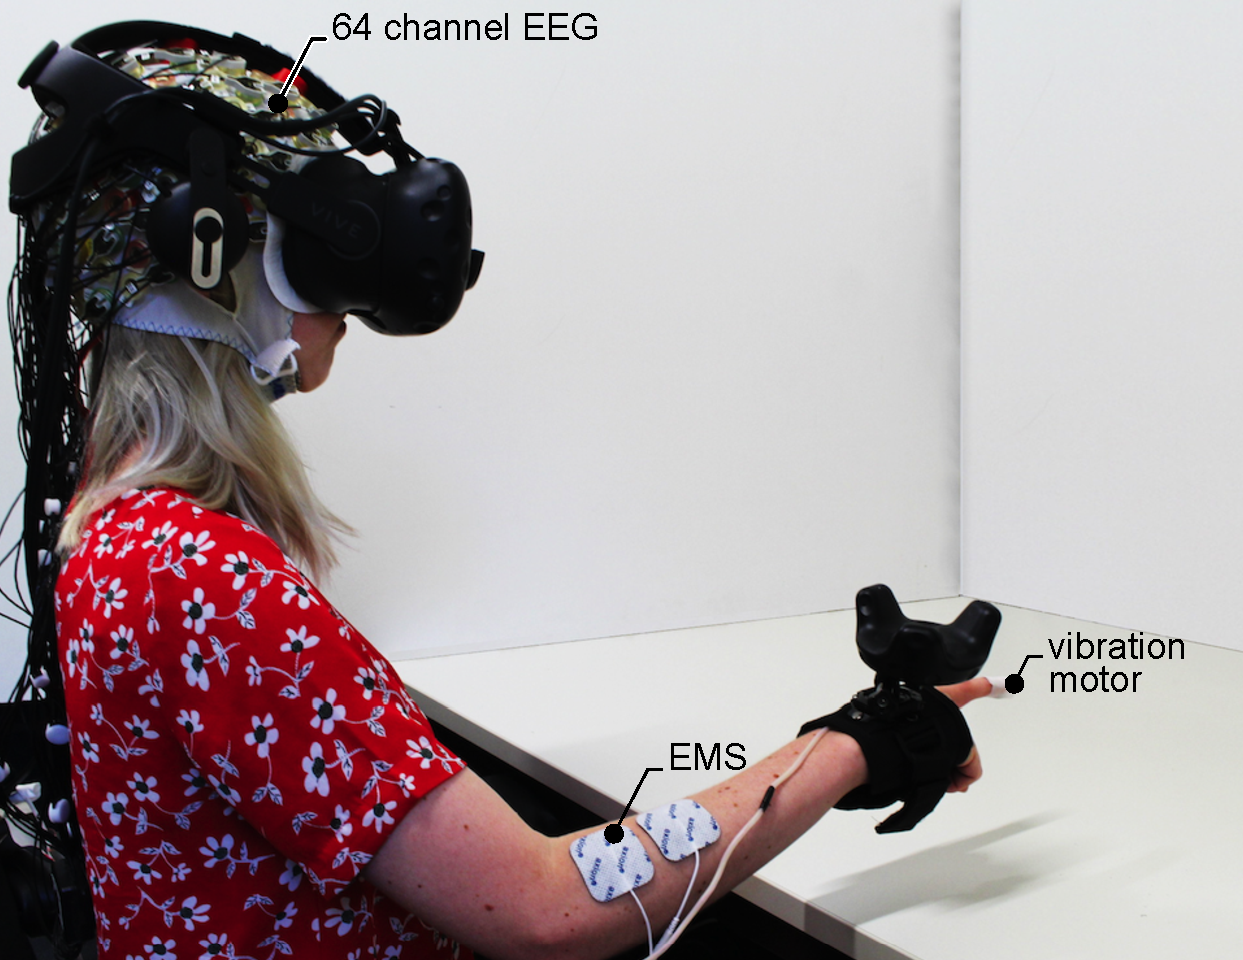
\includegraphics[width=\linewidth]{figures/experiment.pdf}
%\missingfigure[figcolor=white]{Shows setup.}
%\vspace{-17pt}
\caption{Our experimental setup (image with consent from participant).}
\label{setup}
\end{figure}

\textbf{(1) VR and hand tracking.} We used an HTC Vive headset (HTC Corporation, Taoyuan, Taiwan) with the Vive Deluxe Audio Strap and custem EEG cap spacers \footnote{https://grabcad.com/library/adapter-for-vr-eeg-setups-1} to ensure a good fit and less discomfort due to the EEG cap. We used a Vive Tracker, attached to the participant's wrist, to track their right hand. 

\textbf{(2) Vibrotactile feedback.} We used a vibration motor (Model \textit{308-100} from \textit{Precision Microdrives}), which generates 0.8g at 200Hz. This motor measures 8mm in diameter, making it ideal for the fingertip. The vibration feedback was driven at 70mA by a 2N7000 MOSFET, which was connected to an Arduino output pin at 3V.

\textbf{(3) Force feedback.} We actuated the index finger via electrical muscle stimulation (EMS), which was delivered via two electrodes attached to the participants' \textit{extensor digitorum} muscle. The finger actuation was achieved via a medically-compliant battery powered muscle stimulator (\textit{Rehastim} from \textit{Hasomed}), which provides a maximum of 100mA and is controllable via USB. 

% We utilized the extensor digitorum since we found that we can robustly actuate it without inducing parasitical motion of neighboring muscles; this was verified during pilot studies. This finger actuation was achieved via a medically-compliant battery powered muscle stimulator (\textit{Rehastim} from \textit{Hasomed}), which provides a maximum of 100mA and is controllable via USB. We chose this device since it had been successfully used by researchers as a means to generate force feedback in both VR~\cite{lopes_walls_2017} and AR~\cite{lopes_AR}. The EMS was pre-calibrated per participant to ensure a pain-free stimulation and robust actuation. 

\textbf{(4) EEG Setup.} EEG data was recorded from 64 actively amplified electrodes using BrainAmp DC amplifiers from BrainProducts. Electrodes were placed according to the extended 10\% system ~\cite{oostenveld_five_2001}. After fitting the cap, all electrodes were filled with conductive gel to ensure proper conductivity and electrode impedance was brought below 5kOhm for all electrodes. EEG data was recorded with a sampling rate of 1000 Hz. We synchronized tracking, EEG data, and an experiment marker stream that marked sections of the study procedure using labstreaminglayer\footnote{https://github.com/sccn/labstreaminglayer}.

\begin{figure*}[!ht]
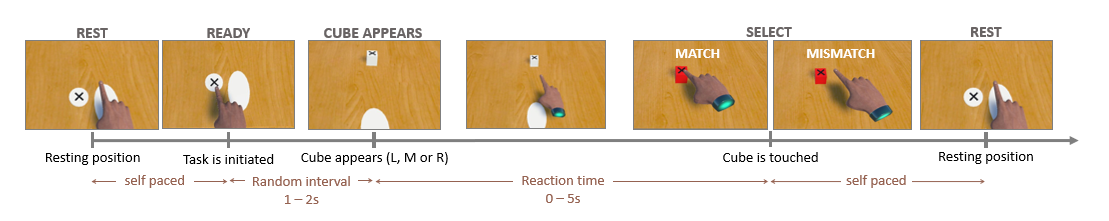
\includegraphics[width=\linewidth]{figures/Task_mismatch.PNG}
\vspace{-15pt}
\caption{Interaction flow depicting one trial in our 3D object selection task.}
\label{task_flow}
\end{figure*}

\subsection{Training phase}
We asked participants to wear the HTC VIVE VR headset for a maximum of 24 trials practice trials. Overall, the EEG fitting, calibration, and practice trials took around 30 minutes (with two experimenters).

\subsection{Task}
Participants performed a 3D object selection task in VR design with Unity Software (Unity Technologies, San Francisco, USA). The interaction flow of our task, depicted in Figure~\ref{task_flow}, was as follows: (1) participants moved their hands from the \textit{resting position} to the \textit{ready position}, to indicate they were ready to start the next trial; (2) participants waited for a new target to appear (the time of a new target spawning was randomized between 1-2 s); (3) then, the target (a cube) would appear in one of three possible positions (center, left, right), all equidistant from the participant's \textit{ready position}; (4) then, participants acquired the target by moving and touching the target with their index finger. (5) After a target was acquired, participants moved back to the \textit{resting position}. Here, they could take a break before the next trial.

\subsection{Interface conditions}
Participants performed the task in three additive feedback conditions:

(1) \textbf{visual-only (Visual)}: when participants touched the cube, it changed its color from white to red (visual feedback)
% ; our no-haptics \textbf{baseline}~\\
\indent(2) \textbf{tactile (Vibro)}: when participants touched the cube in the vibro condition, they received a 100 ms vibroactile stimulus and the color change (visual + tactile feedback)
% ; this is the only available haptic feedback in today's VR experiences.~\\
\indent(3) \textbf{force-feedback (EMS)}: in this condition, participants also received a 100 ms of EMS stimulation at the index finger extensor in addition to the visual and vibrotactile feedback (visual + tactile + force feedback)
% . As prior research showed the EMS stimulation of the opposing muscle (in our case, the extensor) is perceived as the resisting force that arises from pushing against the cube (i.e., force feedback)~\cite{lopes_muscle-propelled_2013,lopes_walls_2017,lopes_impacto:_2015}.

% We designed our three feedback conditions additively because additional haptic feedback is generally associated with more haptic realism, therefore, we hypothesized that ERPs would demonstrate some correlation to the ascending level of the feedback's realism.

\subsection{Introducing Visuo-Haptic Mismatches}
To allow us to compare the event-related EEG and movement signatures in a realistic vs. unrealistic interaction, we presented participants with two different classes of trials: \textbf{match trials (C)} (75\% of the trials) and \textbf{mismatch trials (M)} (25\%). This procedure elicits a prediction mismatch signal in 25\% of the trials similar to previous designs investigating the impact of target probabilities~\cite{polich_updating_2007}.  %on ERP modulations
In the \textbf{matching} trials, the feedback stimuli were presented upon touching the object, exactly when participants expected them to occur based on the available visual information (finger touching the target). In contrast, in the \textbf{mismatch} trials, the feedback stimuli were triggered prematurely, which was accomplished by enlarging the invisible radius of touch detection by 350\%. While in the match trials, we used a cube collider of the exact size of the VR cube, in the mismatch trials, we used a larger sphere collider. Our collider enlargement was based on the study design by Singh et al.~\cite{singh_visual_20008}, in which they showed that VR users can detect a visual mismatch at around 200\% of offset from the target. In our pilot tests, we decided to extend the offset to 350\% to make the mismatch more obvious so as to provoke more pronounced prediction errors. 

Also, we used a match-to-mismatch ratio of 75\%-25\% of the total trials by modeling our study after previous studies, which also ensure that participants are faced with a detectable unrealistic behavior of the virtual environment~\cite{Liao2011,Wiersema2007,Donchin1988}. For these unrealistic trials to occur, the participants must first be able create a stable model of how the VR world operates, thus the VR world cannot behave at a random 50\%-50\% match-mismatch ratio.

Finally, these match vs. mismatch trials were presented in five randomly generated sequences, each with an equal distribution of matches and mismatches.

\subsection{Experimental design}
The experiment consisted of five phases: (1) a setup phase; (2) a calibration phase; (3) a short training phase; (4) the task itself, in all three possible interface conditions, each followed by a subset of items from the IPQ questionnaire (G1, REAL2, SP4 and INV1)~\cite{T.W.Schubert2003} and the NASA-TLX~\cite{Hart1988}. Lastly (5) participants were asked about their experience in the VR and which condition they enjoyed the most.

% For completeness, at the end of each condition we presented the four most relevant questions from the standard IPQ~\cite{ipq_paper}, in particular: G1, REAL2, SP4 and INV1. However, our hypothesis was that the inclusion mismatch trials, which were presented in 25\% of the cases, would lower the IPQ ratings dramatically.

We used a within-subjects design with 300 trials for each, the Visual and Vibro feedback condition, and 100 trials for the EMS condition. The order of the Visual and Vibro conditions was randomized across participants with the EMS condition always being the last block. 
% This was done to avoid potential overshadowing of the EMS stimulation (a very strong sensation) on the two other stimulation conditions.





%%%%% resources:
% \subsection{Task and Procedure}
% Using an HTC Vive VR Headset with the Vive Deluxe Audio Strap and a Vive Tracker (HTC Corporation, Taoyuan, Taiwan) attached to the right hand, a 3D object selection task was presented on a virtual table placed on an infinite white plane. The virtual environment was created in the Unity3D engine (Version, company details). White cubes appeared at random either in the center, to the left, or to the right of the participant, equidistant from a starting position (see Figure ??). The time of a new cube spawning was randomized between 1-2 seconds after starting a trial. 

% %no subsections? This so hard to parse, make a task heading or so?
% Participants were tasked to select the cube with their index finger and, upon completion, move their hand back to a resting position indicated on the table. The task was completed in two blocks of 300 trials each, with one block providing visual-only feedback, i.e. the cube changing its color from white to red upon selecting, and one block providing visual-tactile feedback, in which the selection contact was indicated by the color change plus a small vibrotactile pulse. Placed under the index fingertip, a vibration motor (Model \textit{308-100} from \textit{Precision Microdrives}), generating 0.8g at 200Hz and measuring 8mm in diameter was driven at 70mA by a 2N7000 MOSFET connected to an Arduino output pin at 3V. An initial 24 trial training session was followed by the two experimental blocks (balanced across participants), each followed by two questionnaires, NASA-TLX and IPQ. For the main experimental manipulation of asynchrony, 25\% of the trials (totalling 75 asynchronous trials per feedback block of 300 trials) exhibited spatio-temporal asynchrony in line with established oddball paradigms. Object selection was triggered prematurely by bounding a spherical collider to the cube and enlarging it by 350\% in comparison to a collider bounded to the shape of the cube in the synchronous trials. Asynchronous trials were sorted in a pseudo-randomized sequence following synchronous trials, i.e. between one and five synchronous trials preceeded an asynchronous trial. Extended task and apparatus descriptions can be found elsewhere \cite{Gehrke2019}.
% % todo add movie, figure and references
\subsection{Dataset}
\subsubsection{Participants}
20 participants (12 female, mean age = 26.7 (sd = 3.6)) were recruited through an online tool provided by the Department of Psychology and Ergonomics and through local listings. Participants were right-handed, had normal or corrected to normal vision and had not experienced VR with either vibrotactile feedback at the fingertip or any form of force feedback, including EMS. Participants were compensated with 10 Euros per hour or study credits. Participants were informed of the nature of the experiment, recording and anonymization procedures and signed a consent form approved by the local ethics committee of the Department of Psychology and Ergonomics at the TU Berlin. Data of the first subject had to be removed from further analyses due to data recording error. 

% TODO:
% [] add ethics approval credentials

\subsubsection{Recordings: Motion Capture and EEG}
EEG was recorded using 64 active Ag/AgCl electrodes placed according to the extended international 10–20 system \cite{Chatrian1985a}. The electrode at position FP2 was detached from the cap and placed under the left eye to provide additional information about eye movements (EOG). Impedance was kept under 30 \si{\kohm} and the EEG was sampled at 500 Hz and amplified using BrainAmp DC amplifiers (Brainproducts GmbH, Gilching, Germany). Hand and head movements were sampled at 90 Hz when coming out of the HTC Vive processing cascade. Samples were recorded and synchronized using labstreaminglayer \footnote{https://github.com/sccn/labstreaminglayer}.

\subsubsection{Reproducing Results and Data Availability}
Data, experimental protocol, analyses code and earlier publications are accessible from a comprehensive repository hosted at open science foundation (OSF)~\footnote{https://osf.io/x7hnm/}. BIDS formatted data is hosted on openneuro~\cite{} and a full reproduction of the presented results is feasible.

% TODO
% [] add citation to openneuro dataset
\subsection{Processing}

\subsubsection{Brain activity: EEG Preprocessing, Independent Component Analysis (ICA)}
EEG data preprocessing and ICA were performed in Matlab 2019b (MATLAB, The MathWorks Inc., Natick, MA, USA), using EEGLAB toolbox \cite{Delorme2004a} and custom 'BeMoBIL Pipeline' scripts and functions \footnote{https://github.com/BeMoBIL/bemobil-pipeline}. Single subject data were lowpass filtered with 124Hz and subsequently down-sampled to 250Hz. Channels which were contaminated with artifacts were automatically rejected using the PREP pipeline \cite{Bigdely-Shamlo2015} 'FindNoisyChannel' function, which is selecting bad channels by amplitude, the signal to noise ratio and correlation with other channels. Rejected channels were then interpolated while ignoring the EOG channel, and finally re-referenced to average reference (data A). The data was then filtered with a 1 Hz highpassfilter (data B) and a first adaptive mixture independent component analysis, AMICA \cite{Palmer2011}, was used to identify eye related independent components (ICs) which were projected out of the sensor data. For this, the rank was reduced by one for average reference use and further by the number of interpolated channels in the respective data set. To identify eye components, IClabel \cite{Pion-Tonachini2019} was used, whereas components exceeding a value of 0.7 for the 'eye' class were defined as eye components. Then, to detect segments of noisy data, an automated time domain cleaning (see \citet{Gramann2018}) was performed on narrowly filtered data from 1 to 40 Hz. The data was therefore first split into 1 second long segments for which the mean absolute amplitude and standard deviation of all channels as well as the Mahalanobis distance of all channel mean amplitudes were calculated. All three methods results were then joined together in order to rank all segments. The 12\% highest ranking noisy segments were selected for rejection and an additional buffer of $\pm 0.49$ sec was added around each segment resulting in about 15\% rejected data for each subject. This data was rejected from data B and a second AMICA was calculated on this time domain cleaned data. A dipole fitting procedure was performed for each spatial filter using the 10-20 standard electrode locations and a boundary element head model (BEM) based on the MNI brain (Montreal Neurological Institute, MNI, Montreal, QC, Canada). The spatial filter information was then copied back to the preprocessed, interpolated and average referenced data set (data A). 

Ultimately, all ICs with a probability smaller than .7 as indicated by the ICLabel 'brain' class were projected out of the data resulting in the final dataset of very likely brain sources and their projections to the channels investigated in all subsequent analyses. Across the study set, 271 independent components were retained forming a representative sample of about 14.3 (sd = 5.0) components per participant. 

\subsubsection{Behavior: Motion Capture}
Motion capture data was filtered with a 6Hz lowpass filter and upsampled to match EEG frequency using MoBILAB routines for concurrent analyses \cite{Ojeda2014}. Subsequently the first derivative was computed and velocity was extracted. 

We assessed post-error adaptation as a function of change in 'action time': the time elapsed between the start of the reaching movement following object spawn and the end of that movement. The reach onset was detected by stepping back from the peak velocity of the reach and selecting the first sample where the velocity fell below 0.05 m/s. The end of the reach was determined as the first sign change of the change in z-direction, the primary reach direction, following the start of the reach. Trial-to-trial changes in action time were computed to assess the effectiveness of the experimental manipulation~\cite{Dutilh2012}. As such, action time was independent from the too-early appearance of the mismatch feedback. 

We modeled the occurrence of mismatch trials with a linear mixed effects model employing the trial-to-trial change rate in action time. The model $mismatch ~ change_in_action_time + (1 | participant_id)$ was fit using Matlab's 'fitglme' function. The predictive accuracy of the model was assessed using 10-fold cross-validation. To assess the models effectiveness, a two-sample ttest was computed using each fold's accuracy and the simulated chance level considering the the classes sample size in each fold~\cite{Muller-Putz2007}.

\subsubsection{EEG Classifier, Classifier Scalp Projections and Localization of Components relevant to Classification}
Following \citet{Zander2016} a regularized linear discriminant analysis classifier was trained per participant with all mismatch trials constituting class 1 and a random sample of an equal size of match trials labeled class 2. Using the open-source toolbox BCILAB ver. 1.4 the classifier was trained on windowed means as features. First, EEG data were re-sampled to 100 Hz and band-pass filtered from 0.1 to 15 Hz. Average amplitudes of all channels in eight sequential 50 ms time windows between 50 and 450 ms after the cube was touched were extracted, the windowed means feature vectors. A mean baseline taken in the 0 to 50 ms window post event was subtracted in order to compensate for event classes, match and mismatch, occurring at different stages of the ongoing movement. For robust performance estimation, a 5 x 5 nested cross-validation was used to calculate the classifiers reliability. Classification accuracy was statistically evaluated using a two-sample ttest with the mean classifier accuracy per participant across folds and simulated chance level given trial numbers in each class \cite{Muller-Putz2007}.

In order to learn what regions of the brain the classifier specifically relied on, we first transformed the LDA filters at each time window to LDA patterns reflecting a mixture of scalp activations with regards to the discriminative source activity. Subsequently, the relevance for classification can be computed using LDA filter weights per time window and the ICA umixing matrix \cites{Haufe2014a, Zander2016}. The equivalent current dipole models of independent components were then weighted by their relevance and ultimately visualized via EEGLAB dipoleDensity plots \cite{Krol2019}. 

\subsection{Mismatch processing in midcingulate independent components}
We established a \textit{highest relevance for classification} voxel via visual inspection at $[0, -35, 50]$ (in MNI space, reflecting a source located in or near the superior parietal, BA40) used as a seed region of interest (ROI) for targeted optimization of group-level IC clustering.

% TODO adapt new solutions ROI here

\subsubsection{Clustering Independent Components}
To allow for group-level analyses across independent components, we clustered components based on their equivalent dipole locations using a region of interest (ROI) driven repetitive k-means clustering approach \cite{Gramann2018}. ICs were clustered by applying the k-means algorithm with k equals 14, the median number of ICs retained across participants. ICs with a distance of more than three standard deviations from any final centroid mean were considered outliers. After applying desirable weights (number of participants: 2, ICs/participants: -2, spread: -1, RV: -1, distance from ROI: -2, Mahalanobis distance from the median: -1) the optimal target cluster 

% TODO adapt clustering solution here

solution contained 21 ICs from 17 participants, that is a ratio of ~1.2 ICs per participant, a normalized spread (mean squared distances from individual dipoles to cluster centroid) of 371.8 $mm^2$, a mean RV of 5.8\%, and a distance of 5.1$mm$ to the ROI. Four participants exhibited two ICs contained in the optimized cluster. We chose to average their activity following the assumptions of our clustering approach.

\subsubsection{Modeling Event-related Spectral Perturbations}
To keep all task events from cube spawn to touch, data were epoched -3 to +2 seconds around the 600 cube touches and trials were removed if (a) the reaction time between cube \textit{spawn} and touch exceeded two seconds or (b) large voltage fluctuations in the channels were detected via EEGLABs \textit{autorej} function with default settings.

% TODO add epoch removal info and modeling, mcc approach

On average 83.7 (sd = 37.6) trials were removed. For the clean single trials we computed event-related time-frequency decompositions (event-related spectral perturbation, ERSP) of each independent component time course. Time-frequency decomposition were computed via the \textit{newtimef} function in EEGLAB for 3 to 80 Hz in logarithmic scale, using a wavelet transformation with 3 cycles for the lowest frequency and a linear increase with frequency of 0.5 cycles. Subsequently, phase was discarded, the output squared and resulting raw power values kept for further analysis.

To obtain first-level, per participant, summaries of ERSP, mass-univariate multiple regression was computed across all mismatch trials. Therefore, a linear model was estimated at each time-frequency pixel of participants independent component(s) present in the ROI cluster. The linear model was defined as \textit{tf\textunderscore pixels = intercept + match\textunderscore mismatch * haptic\textunderscore feedback + baseline}. Match\textunderscore mismatch differentiated match trials from mismatch trials and haptic\textunderscore feedback vibrotactile from those missing the added immersive channel. To further infer whether components of the event-related response could be explained by baseline activity, average power per frequency bin in the -200 to 0 ms window preceding cube \textit{spawns} was entered as a predictor as well.

% TODO sample size in ROI cluster(s)

For inference, a permutation t-test using EEGlab's \textit{statcond} function with 1000 permutations was employed on the regression betas. Due to the small sample size in the ROI cluster (N = 14) we chose the permutation-t approach over a cluster statistic with constrained resampling for multiple comparison correction~\cite{Pernet2015}. First, for each permutation the betas map of t-scores was transformed to a map of tfce-scores. Next, for each tfce-map the maximum was extracted and the true tfce-map was thresholded at the 95th percentile of the max-tfce distribution from the 1000 permutations. 





%%%%% resources
% \subsubsection{Modeling Event-related Spectral Perturbations in "Midcingulate" Independent Components}
% % Linear modeling of Clusterwise Event-related Spectral Perturbation
% % specify the model and briefly state to what end it was designed, which questioned it was supposed to answer 

% \subsubsection{Single-Trial Multiple Regression, Group-level Statistics and Multiple Comparison Correction}
% In order to describe task execution relevant components of the event-related spectral perturbations of the entire epoch, we conducted a t-test of the grand average cluster ERSP, baseline corrected using grand average divisive baseline. Employing a permutation t-test using the function \textit{statcond} with 1000 permutations we controlled for multiple comparisons. Due to the small sample size (N = 17) we chose the permutation-t approach over a cluster statistic with constrained resampling \cite{Pernet2015}. This procedure was also used to assess inference of betas obtained from mass-univariate single-trial regressions as described below. With respect to the grand-average, slight shifts preceding the event of interest due to randomized pre-trial intervals were ignored and averaged across. This smearing in time was accepted since time-frequency resolution similarly reduces temporal accuracy. Since single-trial analysis only focused on the interval succeeding the event of interest, that is the feedback associated with touching the cube or, in case of mismatch trials, the premature feedback, randomized pre-trial intervals did not impact these analyses.
% % todo % citation statcond (fieldtrip and eeglab)
% %In order to correct for multiple comparison we transformed the resulting map of t-scores to a map of tfce-scores and thresholded the tfce-map at the 95th percentile of the max-tfce distribution of 600 bootstrapped t-tests using as implemented in LIMO EEG. Due to the low number of 17 participants in each analysed cluster, we constrained bootstraps to contain at least 14 unique participants to overcome conservative multiple comparison correction \cite{Pernet2015}.

% % better split grand-average and single-trial analyses
% \subsubsection{Single-trial regression to disentangle spatio-temporal binding prediction errors}
% To obtain first-level, per participant, summaries of event-related spectral perturbations, mass-univariate multiple regression was computed across all mismatch trials. Therefore, a linear model was estimated at each time-frequency pixel of participants independent component(s) present in the ROI cluster. The linear model was defined as \textit{tf\textunderscore pixels = intercept + hand\textunderscore velocity * haptic\textunderscore feedback + RT + Baseline}. Instantaneous hand velocity was extracted at the moment of object selection. Haptic feedback differentiated trials including vibrotactile from those missing the added immersive channel. In order to estimate the interaction term between hand velocity and haptics, both predictors were normalized prior to model fitting. Reaction time was operationalized as the time elapsed from the object spawning on the table to the object being selected. To further infer whether components of the event-related response could be explained by baseline activity, average power per frequency bin in the -200 to 0 ms window preceding cube \textit{spawns} was entered as a predictor as well.
% %optional if results are promising -> \subsection{correlation post-error slowing and theta}

% \subsubsection{Velocity perturbations following spatio-temporal binding prediction errors}
% To investigate whether ongoing motor behavior following spatio-temporal binding manipulations changed as a function of time or in response to haptic feedback a mass-univariate multiple regression was computed across all mismatch trials. The linear model \textit{velocity = intercept + trial\textunderscore number * haptic\textunderscore feedback} was fit at all time points addressing whether (a) trials were comparable across time and (b) whether rendering the surface by means of tactile feedback impacted movement execution potentially hinting at perceived object rigidity. At the group-level, a robust one-sample t-test was computed for betas of trial number and haptic feedback. To assess whether initiation and motor execution slowed down following spatio-temporal binding perturbations per participant betas were obtained by fitting the linear model \textit{velocity = intercept + following\textunderscore asynchrony * following\textunderscore haptics} at all time points across the epoch followed by group-level inference as described above.

% no overlapping ICs in clustering twice, one parietal, one visual association
% old solution
% (weight=6), grand-average ERSPs (weight=3), mean log spectra (weight=1), and scalp topography (weight=1),
 %The weighted IC measures were reduced to a 10-dimensional feature vector for clustering via PCA. 
 
 % maybe add movie for supplement material
% todo cite dipoledensity
%\footnote{Available at https://sccn.ucsd.edu/wiki/EEGLAB_ Extensions_and_plug-ins}
%and $[20, -65, 30]$ 
% make clear that class size was subsampled

% On average 83.7 (sd = 37.6) trials were removed. For each remaining single trial we considered event-related potentials for channels and independent components (ERP), event-related velocities, i.e. the magnitude of velocities in x, y and z direction (ERV) as well as event-related time-frequency decompositions (event-related spectral perturbation, ERSP). Time-frequency decomposition were computed via the \textit{newtimef} function in EEGLAB for 3 to 80 Hz in logarithmic scale, using a wavelet transformation with 3 cycles for the lowest frequency and a linear increase with frequency of 0.5 cycles. Subsequently, phase was discarded and raw power values were kept for further analysis. Where applicable, grand average ERSPs are computed by first averaging both trial data and baselines across trials in power then dividing trial data by baseline and transforming the outcome to logarithmic scaling ($dB = 10*log_{10}(power)$). ERPs are plotted after bandpass filtering with a low and high cutoff at 0.1 and 15 Hz respectively.


% % results

\section{Results}

Participants reached towards the target object after it appeared, `spawned', on the table. In the match trials without visuo-tactile glitches, participants took on average 1.04s (SD = .19) to complete the reach-to-touch. In the mismatch trials with visuo-tactile glitches, the target feedback was presented prematurely and triggered on average after .73s (SD = .12) following object spawn, see figure 1b. Hence, increasing the (bounding) object volume for collision detection led to a spatio-temporal mismatch of approximately 300 ms as compared to the congruent condition. The velocity profile in both conditions exhibited a narrow peak during outward reaching with a peak magnitude of ~.6 m/s and a broader and lower peak when the hand was retracted back to its origin, see figure \ref{setup_and_behavior}b bottom.

\begin{figure}[!h]
  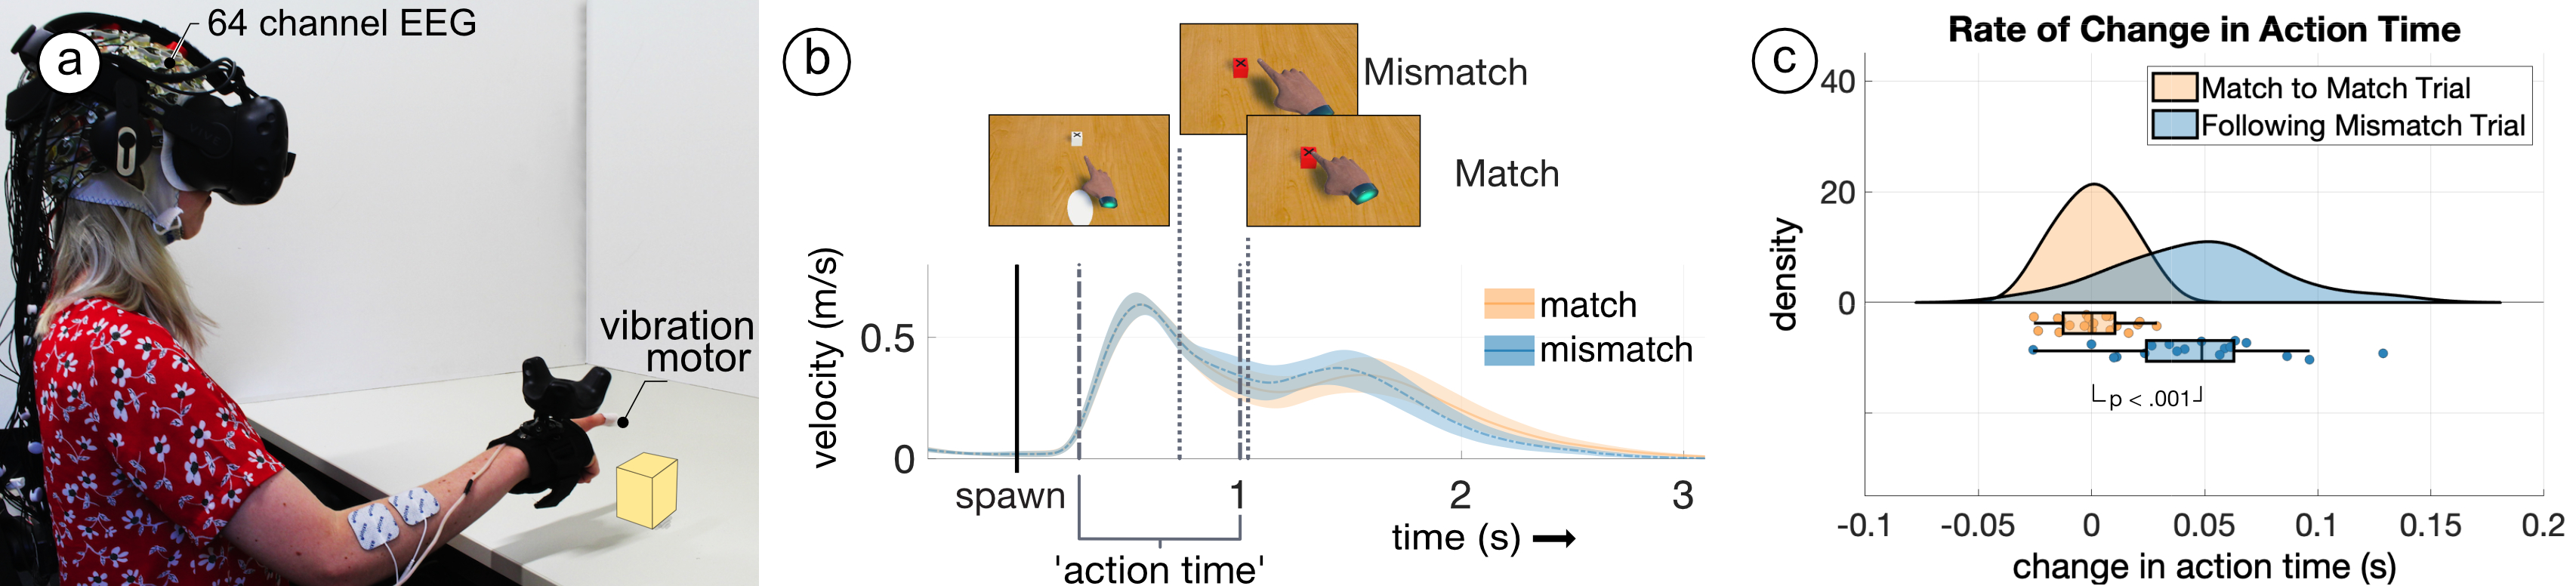
\includegraphics[width=\textwidth]{figures/task_behavior.jpg}
  \caption{Task Structure and hand velocity profile. \textbf{A} Participants were instructed to reach to an appearing cube on a desk in front of them. They were equipped with a VR, a 64 channel EEG cap, electrode spacers and rigid body tracker on the hand. The vibration motor was placed under the fingertip of the index finger. \textbf{B} Top: Inside VR view of experimental scene. Bottom: Grand-average velocity with 95\% confidence interval of both, match and mismatch conditions with event markers for object `spawn', `action time' start and end as well as moments of object touch in match and mismatch conditions. \textbf{C} Distribution of \textit{rate of change} in `action time' between two subsequent match trials and following a VR glitch. A dot represents the average per participant per condition.}
  \label{setup_and_behavior}
\end{figure}

\subsection{Prolonged `Action time' Following VR Glitches}

`Action time', the hand movement period from movement start to reaching the object, lasted on average .74s (SD = .15) in match- and .69s (SD = .15) in mismatch trials. 

% Adding vibrotactile stimulation did not affect hand movement profiles ($b=-.01, t=-1.7, p=.1$) and neither did the interaction of congruity and vibrotactile stimulation ($b=.02, t=1.8, p=.07$). Hence, as with the EEG analysis we pooled trials ignoring the feedback modulation.

We calculated the \textit{rate of change} in `action time' as a metric of post-error slowing. Following match trials, `action time' in the subsequent trial did not change, i.e. 0s (SD = .02). However, following mismatch trials, `action time' was increased in the subsequent trial on average by .05s (SD = .04); this modulation was about 48 times more likely to occur under the model considering mismatch modulation than the null model (equivalent ${\chi}^2_{(1)} = 48.1, p<.001$), see figure \ref{setup_and_behavior}c. 

% Adding vibrotactile feedback did not affect post-error slowing significantly ($b=-.02, t=-1.4, p=.15$). 

Using the trial-to-trial adaptation in `action time', trial classes (match/mismatch) were classified with an average within-subject classification accuracy across folds of 55.4\% (SD = 4.8), remaining below the significance threshold of the simulated chance level at 63.4\% (SD = 0.6).

\footnote{For completeness, we also report a classification scheme using behavioral data of all trials, maintaining unequal trial numbers per match and mismatch condition. We found that using data from all trials and maintaining unequal class sizes increased the classification to 67\% accuracy. See the supplementary material for more detail.}









%%%% writing resources
% Frage: wenn vel profiles mit movement onset aligned dann sollten evtl. kurven gleich sein, es sei denn es gibt einen "kontinuierlichen" rekalibrationseffekt ist in den syncs. mit drin
% im idealfall ist der rekalibrationseffekt 1/4 der 300ms
% Optimierungsprozess um den RMSE bei rekalibration zu optimieren
% mallot VR noise adaptation
% The addition of a haptic sensation while touching the virtual objects (by means of vibrotactile stimulation) led participants to generally move their hand slower during the whole trial, see \ref{setup_and_behavior} C middle row. Participants started their outward movement earlier and their outward peak magnitude was lower when approaching the target (for example at 50 ms preceding object selection, $t_{18} = -2.14, P = .03$). Following trials with spatio-temporal asynchrony, movement behavior was altered in the next trial. An earlier movement onset with a broader peak and immediate retraction following object select was observed (for example at 100 following object selection, $t_{18} = -17.24, P = 0$). Taken together, the task introduced spatio-temporal asynchrony, with rendered vibrotactile feedback as well as the asynchrony impacting future reaching movement characteristics.

\begin{figure}[h]
  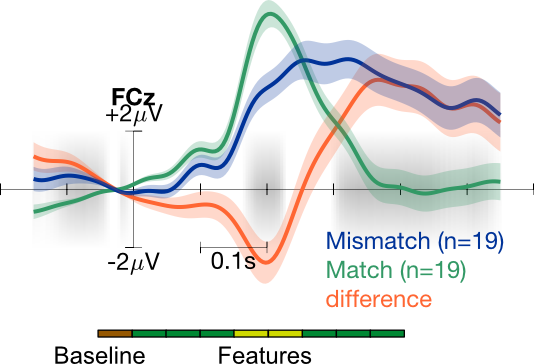
\includegraphics[width=.7\textwidth]{figures/erp_FCZ_diff_delay.png}
  \caption{Grand-average ERP (n = 19) of projected source mixtures at electrode FCz with significant class differences marked in grey. Bottom: Time windows used to compute features for classification (all greens). Windows in light green indicate time windows of interest for classifier source localization.}
  \label{erp}
\end{figure}

\subsection{$\sim$77 \% Classification Accuracy Detecting VR Glitches using ERPs}

We found significant differences between match and mismatch trials in the grand-average event-related potential (ERP) at several scalp locations, see figure \ref{erp} showing the ERP at electrode `FCz' for an example. Hence, we reproduced our previous findings in \cite{Gehrke2019-og} with an altered processing pipeline. At electrode `FCz', amplitude differences at 200 ms indicated a significant difference between mismatch, i.e. the VR glitch condition and the matching trials ($t_{18} = -5.34, p < .001$). Differences were observed most strongly in the 150-280 ms time window, at 250 ms and in later windows starting at 350 ms, see figure \ref{erp}.

To assess the potential for single-trial online applications, a discriminative classification system was cross-validated. The system, using windowed mean ERP features, succeeded in detecting VR glitches. Mismatch and match trials were correctly labeled to the corresponding class with an average accuracy of $\sim$77 percent ($SD = 9.12$). The classification accuracy exceeded chance level at $\sim$ 56 percent, $t_{(18)} = 42.1, p < .001$. 

\subsubsection{Classification Driven by Midline Cingulate and Occipital EEG Sources}

To draw conclusions about the cortical origin of the discriminatory signal we investigated which EEG sources contributed maximally to the classification. With regards to the system's applicability as robust neural interface technology, this source reconstruction served two purposes: (1) Asserting that the classifier did not rely \textit{primarily} on artifact EEG sources, and (2) to gain additional information about the contributing brain regions to allow interpretations about cognitive processing.

In the fourth time window of the eight windowed mean features (150 - 200 ms, see the first light green shaded window at the bottom of figure \ref{erp} and in figure \ref{lda_loc}a top) classifications were driven primarily by activity originating in right lateral parieto-occipital cortical sources (BA19; MNI: x = 30, y = -70, z = 30), see figure \ref{lda_loc}a bottom. In the following time-window (200 - 250 ms, see the second light green shaded window at the bottom of figure \ref{erp} and in figure \ref{lda_loc}b top) the classification signal draw from distributed source activity in occipital areas as well as from sources located in anterior midline cingulate gyrus (near BA23; MNI: x = 0, y = -10, z = 30), see figure \ref{lda_loc}b bottom. Some ocular sources were not classified as such by our automated processing pipeline and carried information relevant to classification in this time window of interest.

\begin{figure}[!h]
  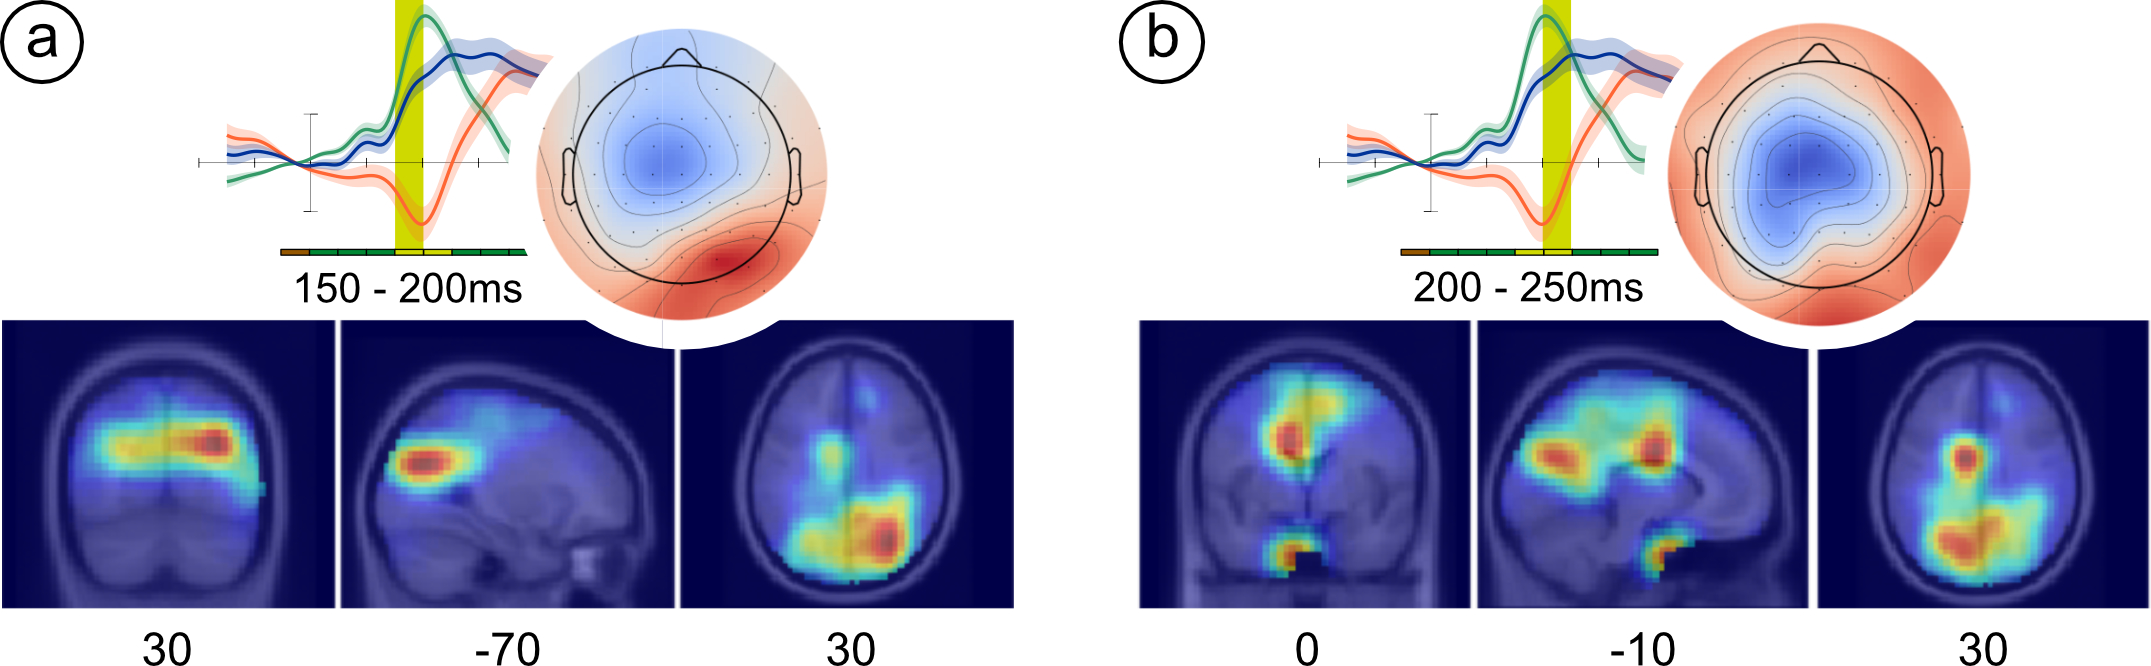
\includegraphics[width=\textwidth]{figures/fig_localization.jpg}
  \caption{An LDA classifier was trained on eight windowed means of 50 ms size from 0 to 400 ms following the cube tap, see figure \ref{erp} bottom. Two classes of synchronous and asynchronous trials were labeled for training and cross-validation. \textbf{a, b} Scalp maps of difference-between-classes activity for the 4th (150-200) and 5th (200-250ms) time windows and the equivalent source localization (MNI coordinates of the location of maximum activity).}
  \label{lda_loc}
\end{figure}

% discussion
\section{Discussion}% start with summary
% aim for 1500 - 2000 words

% Points to discuss
% - is classification success dependent on level of haptic immersion? -> cite that it also works better in meditators for example

Coherent multisensory integration yields meaningful perceptual experiences and is central to adaptive behavior because it allows animals to perceive a world of coherent perceptual entities. In this work, we present evidence for neural signatures originating in central-parietal EEG sources during a spatio-temporal multisensory binding challenge. In order to carve out a signal separating cases of spatio-temporal synchrony from asynchronous cases we employed brain-computer interface technology. Through localization of the classifier weights we gained access to a node in the hierarchical inference network. Subsequent single-trial analysis on the spectral signatures exhibited a separation of alpha- and theta-band characteristics. In the time-domain, the signature can be employed for human-computer interaction purposes as we have shown it is accurately classifiable in two classes. Further, we functionally distinguished theta-band activity from alpha-band activity using single-trial regression. Alpha-band activity following spatio-temporal asynchrony was predicted by baseline activity as well as reaction time, the time elapsed to reach for the target. Both predictors allude to the general temporal task structure and hence may be separated from instantaneous processing. On the other hand, theta-band burst succeeding a binding challenge referred to the multisensory context, that is rendered physics and its interaction with the instantaneous hand velocity.


% maube good conclusion?
Adding to the significant body of evidence about (bayesian) prediction error computations, our findings enable targeted signal acquisition for neural interface technology in VR. 


%%%% writing ressources below
% - discuss reasons for low R^2 and approaches to address it (experiment design and methods (unfolding other processes, adding regressors etc.)) is there a meta study on effect sizes in timefrequency resolved EEG studies. What does Johanna report, regarding effect size?
% - is proprioceptive feedback important in our task: I'd argue against that because I consider vibration on the fingertip to be an exteroceptive sensation and do not consider it relevant where the hand was and how my joints were angled etc. during the mismatch event, therefore i stick to exteroceptive prediction errors only!
% - On world stability: designing visuo-haptic mismatches in virtual environments means further complicating the action-perception cycle understood as hypothesis testing. By pseudo-randomizing when one of the 25 percent chance oddballs appears, hypothesis testing and subsequent evaluation of the latent variables causing the oddball to appear becomes meaningless.

% then summarize results as below paper claim:
%(touch epochs)
%1. LDA location: Central-parietal EEG source activity discriminates between predicted and perturbed visuo-haptic perceptual experiences, in our case the touching of a cube on a desk, baring similarities to a classical simon task.
%(full epochs)
%2.1. ICs clustered to the centroid of the weighted ICs contributing the strongest to the LDA classifier were located to an area between precuneus and posterior cingulate cortex.
%2.2. Hand velocity characteristics, an event-related potential as well as an event-related spectral signature were explained by adding a haptic channel, increasing the level of immersion in the perceptual experience.
%2.3. Further, we observed responses locked to the feedback onset independent of differences in ongoing motor behavior between matching and mismatching classes. (description-level)
%(touch epochs)
%3.1. IC source dynamics following a visuo-haptic perturbation differ from predicted perceptual experiences (see 1., show difference erp and ersp)
%3.2. Following a visuo-haptic perturbation, the context of said perturbation operationalized by hand velocity, haptic feedback and their interaction, impact IC source dynamics only faintly.
%(next trial epochs)
%4. Post perturbation behavioral adaptation is in line with previous findings and may be explainable through reinforcement learning like computations in the brain.

% 1. start with a summary of the most important results
% -> what was the goal of this research?
% 2. situate findings in literature
% -> challenges for mobi research and how to make stimuli more salient
% -> bodily self perception
% 3. link back to introduction and papers cited in introduction

%so there are 2 things participants do in the task: 
%1. they collide too early and immediately adapt hand movement and have mmn / frontal theta -> Prediction Error
%2. they do RL using PE signal and adapt subsequent behavior (trial after mismatch)

% some arguments why ERP:
% - see Cohen 2014 muscle twitches: In our final set of analyses,we examined the ERPs—the time-domain EMG onset-locked EEG potential. Thiswas done mainly to replicate previous findings concerning the relationship between the ERP and partial errors.
% - moving towards an applicable metric to detect things online, hence must be computationally inexpensive, therefore ERPs
% - use ERP section as exemplary for understanding results
% - In haptically richer environments, processing gets more accurate and hence amplifies the error signal originating in or near anterior cingulate cortex (ACC). Moving fast and experiencing richer haptic feedback impact error processing
% - how does erp and ersp correlate. gamma and n200 occipital etc. filtering low frequency for erp does not mean higher ERSP frequency burst might not add to slow cortical ERPs -> therefore, approach is valid

% - discuss with spatial conflict processing: Savoie, & Simon Task results: cohen, cavanagh, toellner
% - reference to self and body ownership, spatial computations between egocentric and allocentric? cite Ehrsson, Slater, Gonzales-Franco (uncanny valley of haptics)
% - single-trial regression challenges in mobile brain body imaging studies: energy of stimulus, Time-locked vs. continuous regressors/stimuli, EEG artifacts due to movement, Contrast desktop stimulation vs. wide FOV in VR, Higher cortical noise, Saliency of stimulus, necessary attention on stimulus %in terms of predictive coding,
% - Study specific shortcomings: low N, both in subjects and in trials due to oddball paradigm
% - assume frontal evaluation of asynchronoy guiding future action and therefore did bot correlate any EEG metric with a post-error slowing parameter.
% - IC sources located near posterior cingulate cortex may anchor the self in the afforded reference frame, providing grounds for spatial predictions during ongoing perceptual experience.

% supplementary material
\section{Supplementary Material}

\subsection{Prolonged `Action time' Following VR Glitches: Leveraging all trials for classification}

Subjecting all trials to the classification scheme, here we report results using the same analysis as in the behavioral part of the results section. Since we leveraged a 75\% to 25\% match to mismatch ratio this increased the amount of data significantly.

`Action time', the hand movement period from movement start to reaching the object, lasted on average .75s (SD = .15) in match- and .69s (SD = .15) in mismatch trials. 

We calculated the \textit{rate of change} in `action time' as a metric of post-error slowing. Following match trials, `action time' in the subsequent trial did not change, i.e. 0s (SD = .01). However, following mismatch trials, `action time' was increased in the subsequent trial on average by .05s (SD = .04); this modulation was about 67 times more likely to occur under the model considering mismatch modulation than the null model (equivalent ${\chi}^2_{(1)} = 67.5, p<.001$), see figure \ref{setup_and_behavior}c.

\begin{figure}[!h]
  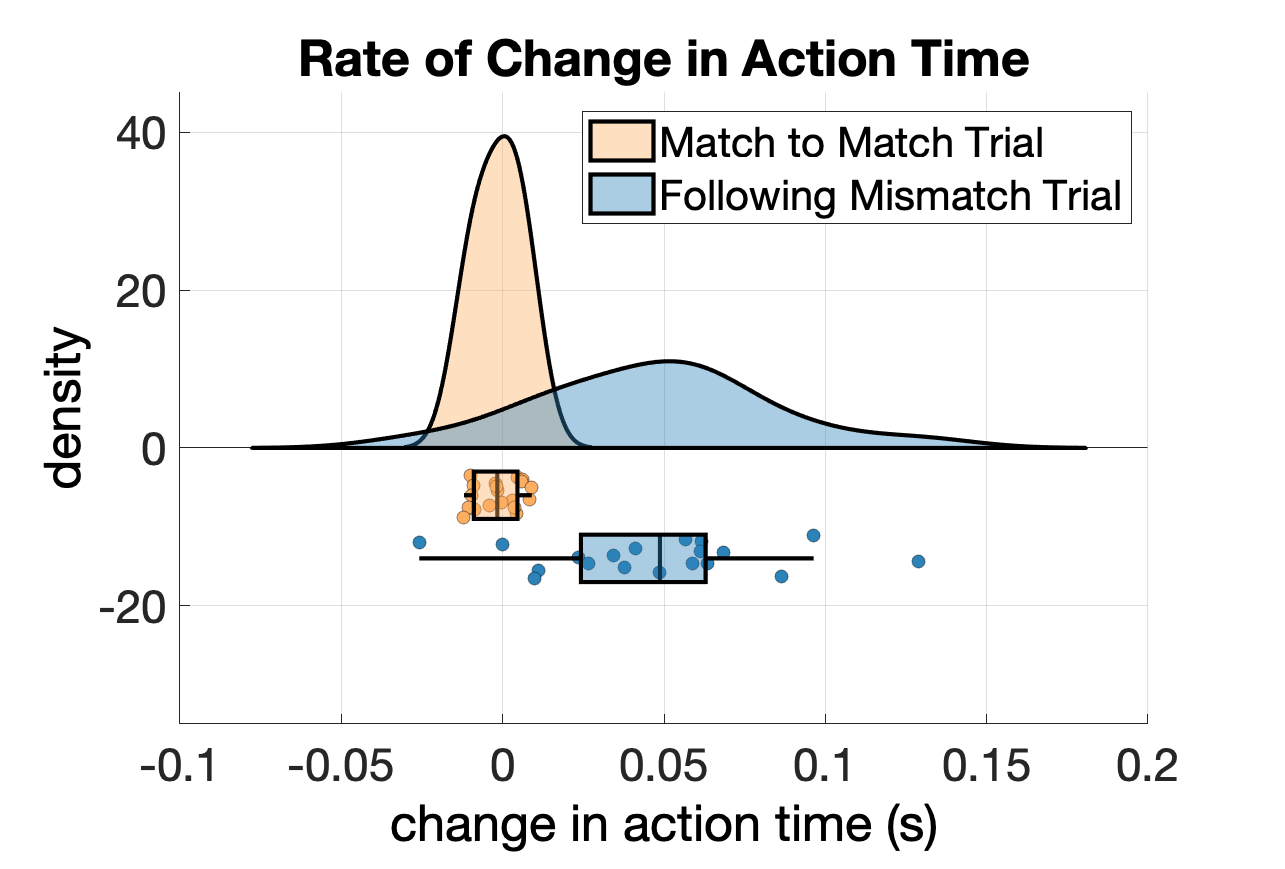
\includegraphics[width=\textwidth]{figures/rate_of_change_action_time_all_trials_.eps}
  \caption{Distribution of \textit{rate of change} in `action time' between two subsequent match trials and following a VR glitch. A dot represents the average per participant per condition. Here, all trial information is considered, maintaining unequal class sizes for match and mismatch conditions.}
  \label{behavior_supplements}
\end{figure}

Using the trial-to-trial adaptation in `action time', trial classes (match/mismatch) were classified with an average within-subject classification accuracy across folds of 67\% (SD = 2.2), exceeding the significance threshold of the simulated chance level at 61.1\% (SD = 0.01, $t_{(18)} = 10.2, p < .001$.

% Submissions are not required to reflect the precise reference formatting of the journal (use of italics, bold etc.), however it is important that all key elements of each reference are included.
\bibliography{references}

\end{document}
